\documentclass[11pt]{article}

\usepackage{fullpage}
\usepackage{graphicx}
\usepackage{amsmath}
\usepackage{amssymb}
\usepackage{amsthm}
\usepackage{fancyvrb}
\usepackage[utf8]{inputenc}
\usepackage{ragged2e}
\usepackage{subfig}
\usepackage{mathtools}
\usepackage{courier}
\usepackage{listings}
\usepackage{booktabs}
\usepackage{multirow}
\usepackage{rotating}


\parindent0in
\pagestyle{plain}
\thispagestyle{plain}


%% UPDATE MACRO DEFINITIONS %%
\newcommand{\horrule}[1]{\rule{\linewidth}{#1}} % Create horizontal rule command with 1 argument of height

\begin{document}

\smallskip

\normalfont \normalsize 
\horrule{0.5pt} \\[0.4cm] % Thin top horizontal rule
{\centering {\huge Experiments design} \\ % The assignment title
\horrule{2pt} % Thick bottom horizontal rule

\linespread{1.5}
\justify

\section{Experiments}

\subsection{Dataset evaluation experiments}
\begin{figure}[h!]
\center
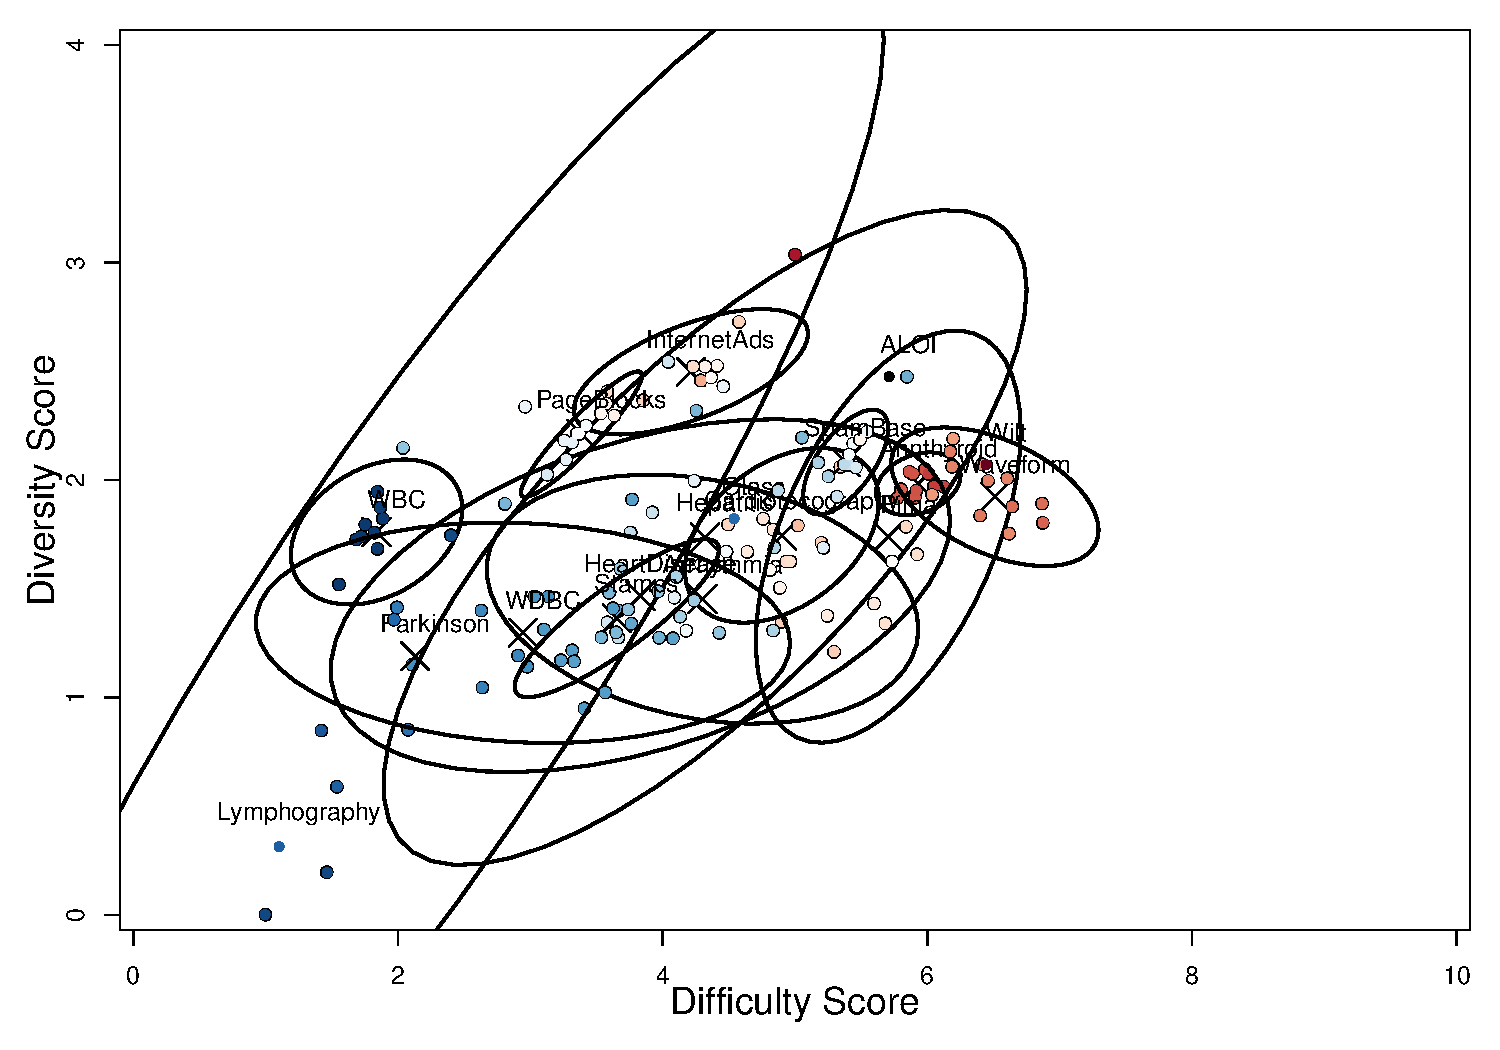
\includegraphics[width=\textwidth]{figs/ellipse_1.pdf}
\captionsetup{justification=centering}
\caption{Diversity Ellipses colored by IREOS ($m_{cl} = 1$). Index not computed for black points.}
\label{fig:DiversityEllipses_1}
\end{figure}
\newpage

\begin{figure}[h!]
\center
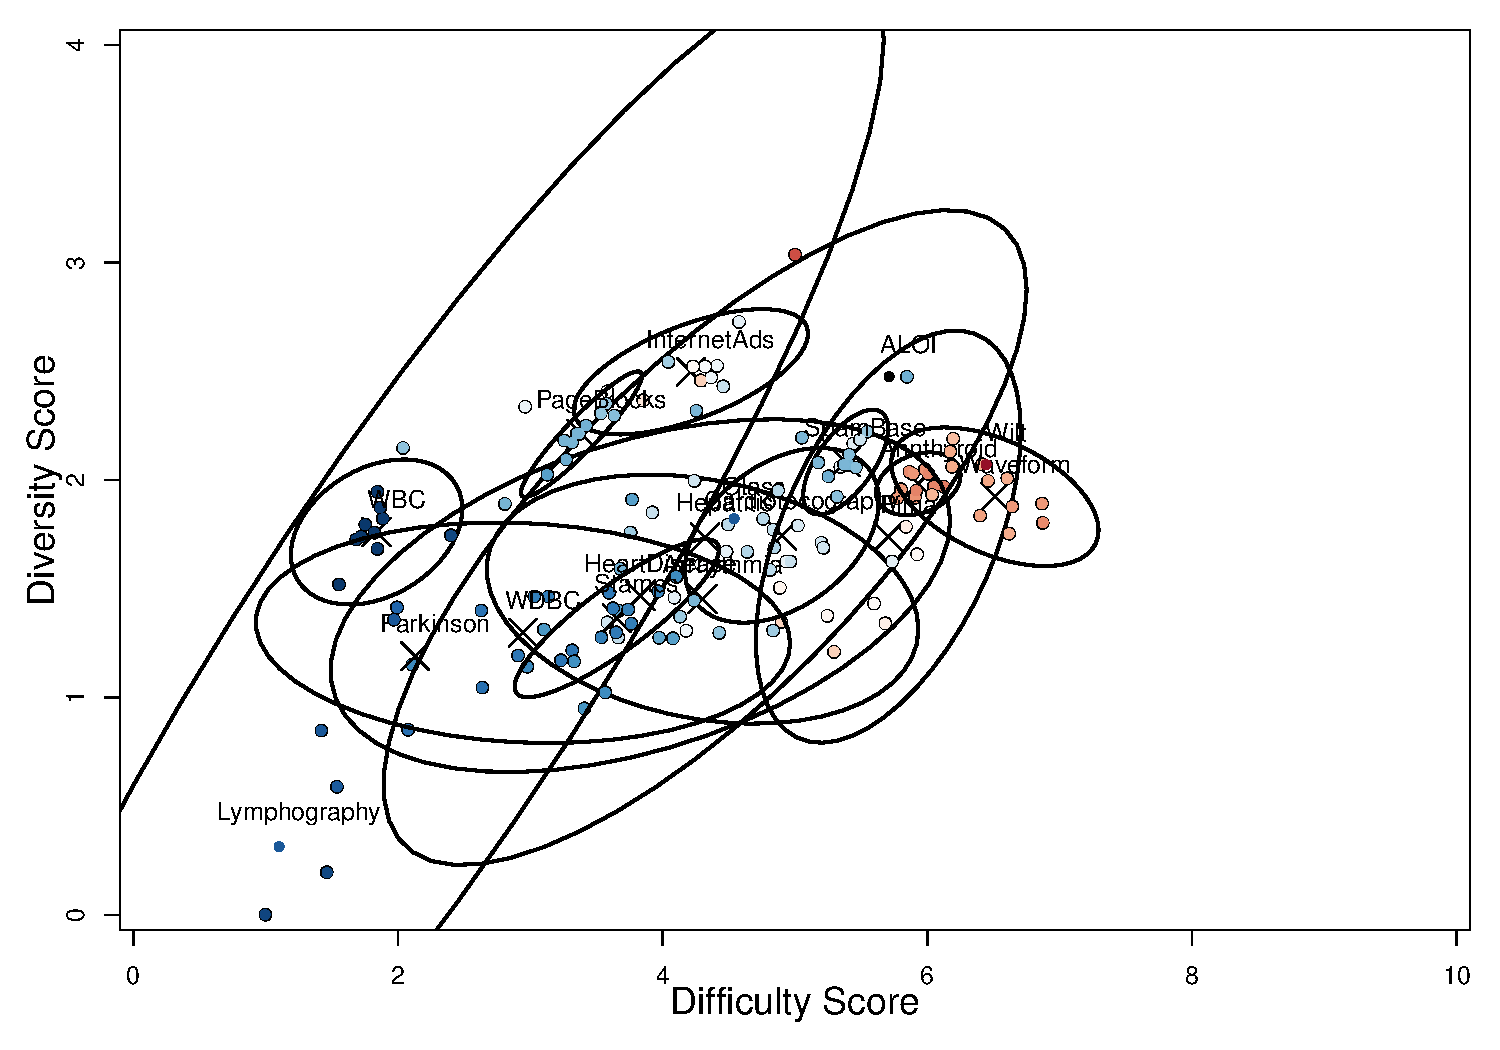
\includegraphics[width=\textwidth]{figs/ellipse_sqrt.pdf}
\captionsetup{justification=centering}
\caption{Diversity Ellipses colored by IREOS ($m_{cl} = \sqrt{5\% of Data Size}$). Index not computed for black points.}
\label{fig:DiversityEllipses_sqrt}
\end{figure}
\newpage

\begin{figure}[h!]
\center
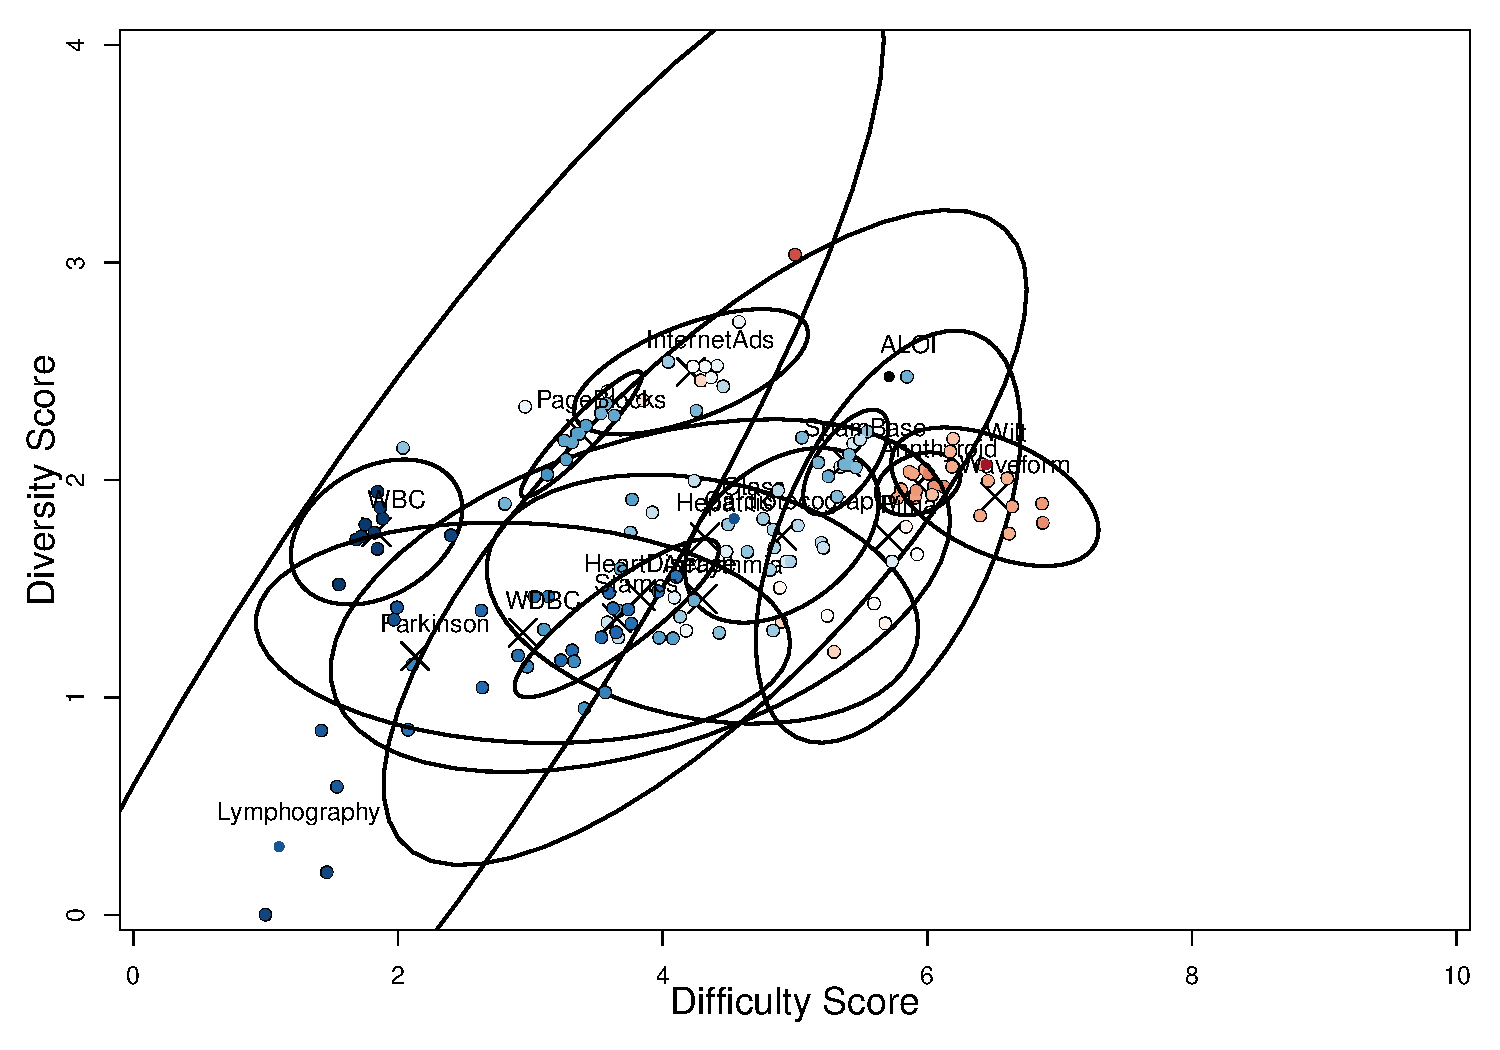
\includegraphics[width=\textwidth]{figs/ellipse_n.pdf}
\captionsetup{justification=centering}
\caption{Diversity Ellipses colored by IREOS ($m_{cl} = n$). Index not computed for black points.}
\label{fig:DiversityEllipses_n}
\end{figure}

\newpage

\subsection{Correlation experiments}\label{sec:cor}
\begin{table}[h!]
\centering
\caption{Spearman correlation}
\label{tab:cor}
\begin{tabular}{llll}
\hline
Dataset 	& $m_{cl} = 1$ & $m_{cl} = \sqrt{}$ & $m_{cl} = n$  \\ \hline
Annthyroid &  -0.079 &  -0.297 &  -0.321  \\
Arrhythmia &  0.588 &  0.697 &  0.697  \\ 
Cardiotocography &  0.685 &  0.976 &  0.988  \\ 
Glass &  0.467 &  0.467 &  0.406  \\ 
HeartDisease &  0.952 &  0.952 &  0.964  \\ 
Hepatitis &  0.939 &  0.927 &  0.927  \\ 
InternetAds &  0.6 &  0.661 &  0.818  \\ 
Lymphography &  0.782 &  0.83 &  0.83  \\ 
PageBlocks &  0.976 &  1 &  0.988  \\ 
Parkinson &  0.6 &  0.6 &  -0.321  \\ 
Pima &  0.745 &  0.952 &  0.855  \\ 
SpamBase &  0.685 &  0.758 &  0.758  \\ 
Stamps &  0.842 &  0.915 &  0.879  \\ 
Waveform &  0.588 &  0.818 &  0.818  \\ 
WBC &  -0.467 &  -0.382 &  -0.418  \\ 
WDBC &  0.309 &  0.309 &  0.309  \\ 
Wilt &  -0.83 &  -0.927 &  -0.927  \\  \bottomrule
\end{tabular}
\end{table}

\begin{table}[h!]
\footnotesize
\centering
\caption{Spearman correlation Synthetic datasets}
\label{tab:corSynt}
\begin{tabular}{llll}
\hline
Dataset     & $m_{cl} = 1$ & $m_{cl} = \sqrt{}$ & $m_{cl} = n$  \\ \hline
gaussian20dim\_4clusters\_nr1 &   1  & & \\ 
gaussian20dim\_6clusters\_nr1 &   1  & & \\ 
gaussian22dim\_5clusters\_nr1 &   1  & & \\ 
gaussian22dim\_6clusters\_nr1 &   1  & & \\ 
gaussian22dim\_9clusters\_nr1 &   1  & & \\ 
gaussian23dim\_4clusters\_nr1 &   1  & & \\ 
gaussian23dim\_9clusters\_nr1 &   1  & & \\ 
gaussian24dim\_2clusters\_nr1 &   1  & & \\ 
gaussian24dim\_3clusters\_nr1 &   1  & & \\ 
gaussian24dim\_4clusters\_nr1 &   1  & & \\ 
gaussian24dim\_7clusters\_nr1 &   1  & & \\ 
gaussian25dim\_5clusters\_nr1 &   1  & & \\ 
gaussian25dim\_9clusters\_nr1 &   1  & & \\ 
gaussian26dim\_4clusters\_nr1 &   1  & & \\ 
gaussian27dim\_5clusters\_nr1 &   1  & & \\ 
gaussian27dim\_6clusters\_nr1 &   1  & & \\ 
gaussian28dim\_4clusters\_nr1 &   1  & & \\ 
gaussian28dim\_7clusters\_nr1 &   1  & & \\ 
gaussian29dim\_3clusters\_nr1 &   1  & & \\ 
gaussian30dim\_4clusters\_nr1 &   1  & & \\ 
gaussian31dim\_4clusters\_nr1 &   1  & & \\ 
gaussian33dim\_3clusters\_nr1 &   1  & & \\ 
gaussian33dim\_5clusters\_nr1 &   1  & & \\ 
gaussian35dim\_6clusters\_nr1 &   1  & & \\ 
gaussian36dim\_8clusters\_nr1 &   1  & & \\ 
gaussian36dim\_9clusters\_nr1 &   1  & & \\ 
gaussian37dim\_3clusters\_nr1 &   1  & & \\ 
gaussian38dim\_9clusters\_nr1 &   1  & & \\ 
gaussian39dim\_2clusters\_nr1 &   1  & & \\ 
gaussian39dim\_5clusters\_nr1 &   1  & & \\ \bottomrule
\end{tabular}
\end{table}


\newpage
\subsection{Model selection experiments}\label{sec:model}

\begin{table}[h!]
\footnotesize
\centering
\captionsetup{justification=centering}
\caption{Summarization of the ROC AUC values for all candidate solutions used in the experiments. Two last columns indicate the solutions selected by ext-IREOS for $m_{cl} = 1$ and $m_{cl} = n$ respectively}
\label{tab:model_selection}
\begin{tabular}{@{}llllllllll@{}}
\toprule
\multicolumn{1}{l|}{Annthyroid} & 0.528 & 0.732 & \multicolumn{1}{l|}{0.63} & 0.642 & \multicolumn{1}{l|}{KNNW} & 0.596 & \multicolumn{1}{l|}{LOF} & 0.551 & \multicolumn{1}{l|}{KNN}  \\ 
\multicolumn{1}{l|}{Arrhythmia} & 0.5 & 0.916 & \multicolumn{1}{l|}{0.737} & 0.879 & \multicolumn{1}{l|}{GLOSH} & 0.879 & \multicolumn{1}{l|}{GLOSH} & 0.879 & \multicolumn{1}{l|}{GLOSH}  \\ 
\multicolumn{1}{l|}{Cardiotocography} & 0.536 & 0.839 & \multicolumn{1}{l|}{0.689} & 0.74 & \multicolumn{1}{l|}{LOF} & 0.806 & \multicolumn{1}{l|}{KNN} & 0.806 & \multicolumn{1}{l|}{KNN}  \\ 
\multicolumn{1}{l|}{Glass} & 0.492 & 0.904 & \multicolumn{1}{l|}{0.699} & 0.539 & \multicolumn{1}{l|}{GLOSH} & 0.539 & \multicolumn{1}{l|}{GLOSH} & 0.539 & \multicolumn{1}{l|}{GLOSH}  \\ 
\multicolumn{1}{l|}{HeartDisease} & 0.387 & 0.97 & \multicolumn{1}{l|}{0.687} & 0.847 & \multicolumn{1}{l|}{KNNW} & 0.847 & \multicolumn{1}{l|}{KNNW} & 0.909 & \multicolumn{1}{l|}{KNNW}  \\ 
\multicolumn{1}{l|}{Hepatitis} & 0.075 & 0.96 & \multicolumn{1}{l|}{0.522} & 0.871 & \multicolumn{1}{l|}{FastABOD} & 0.96 & \multicolumn{1}{l|}{COF} & 0.96 & \multicolumn{1}{l|}{COF}  \\ 
\multicolumn{1}{l|}{InternetAds} & 0.413 & 0.895 & \multicolumn{1}{l|}{0.656} & 0.843 & \multicolumn{1}{l|}{FastABOD} & 0.843 & \multicolumn{1}{l|}{FastABOD} & 0.843 & \multicolumn{1}{l|}{FastABOD}  \\ 
\multicolumn{1}{l|}{Lymphography} & 0.43 & 1 & \multicolumn{1}{l|}{0.748} & 0.847 & \multicolumn{1}{l|}{KDEOS} & 1 & \multicolumn{1}{l|}{COF} & 1 & \multicolumn{1}{l|}{COF}  \\ 
\multicolumn{1}{l|}{PageBlocks} & 0.506 & 0.943 & \multicolumn{1}{l|}{0.728} & 0.896 & \multicolumn{1}{l|}{LOF} & 0.943 & \multicolumn{1}{l|}{LDF} & 0.943 & \multicolumn{1}{l|}{LDF}  \\ 
\multicolumn{1}{l|}{Parkinson} & 0.448 & 1 & \multicolumn{1}{l|}{0.765} & 1 & \multicolumn{1}{l|}{FastABOD} & 1 & \multicolumn{1}{l|}{FastABOD} & 0.625 & \multicolumn{1}{l|}{KDEOS}  \\ 
\multicolumn{1}{l|}{Pima} & 0.499 & 0.834 & \multicolumn{1}{l|}{0.67} & 0.762 & \multicolumn{1}{l|}{LOF} & 0.762 & \multicolumn{1}{l|}{LOF} & 0.762 & \multicolumn{1}{l|}{LOF}  \\ 
\multicolumn{1}{l|}{SpamBase} & 0.463 & 0.779 & \multicolumn{1}{l|}{0.625} & 0.779 & \multicolumn{1}{l|}{KNNW} & 0.779 & \multicolumn{1}{l|}{KNNW} & 0.779 & \multicolumn{1}{l|}{KNNW}  \\ 
\multicolumn{1}{l|}{Stamps} & 0.38 & 0.921 & \multicolumn{1}{l|}{0.655} & 0.921 & \multicolumn{1}{l|}{KNN} & 0.921 & \multicolumn{1}{l|}{KNN} & 0.921 & \multicolumn{1}{l|}{KNN}  \\ 
\multicolumn{1}{l|}{Waveform} & 0.5 & 0.796 & \multicolumn{1}{l|}{0.66} & 0.708 & \multicolumn{1}{l|}{INFLO} & 0.796 & \multicolumn{1}{l|}{LDF} & 0.796 & \multicolumn{1}{l|}{LDF}  \\ 
\multicolumn{1}{l|}{WBC} & 0.438 & 0.997 & \multicolumn{1}{l|}{0.721} & 0.755 & \multicolumn{1}{l|}{LDOF} & 0.755 & \multicolumn{1}{l|}{LDOF} & 0.755 & \multicolumn{1}{l|}{LDOF}  \\ 
\multicolumn{1}{l|}{WDBC} & 0.497 & 0.988 & \multicolumn{1}{l|}{0.745} & 0.884 & \multicolumn{1}{l|}{LOF} & 0.884 & \multicolumn{1}{l|}{LOF} & 0.884 & \multicolumn{1}{l|}{LOF}  \\ 
\multicolumn{1}{l|}{Wilt} & 0.34 & 0.713 & \multicolumn{1}{l|}{0.527} & 0.424 & \multicolumn{1}{l|}{KNNW} & 0.424 & \multicolumn{1}{l|}{KNNW} & 0.424 & \multicolumn{1}{l|}{KNNW}  \\   \bottomrule
\end{tabular}
\end{table}
\newpage
\begin{figure}[ht!]
\center
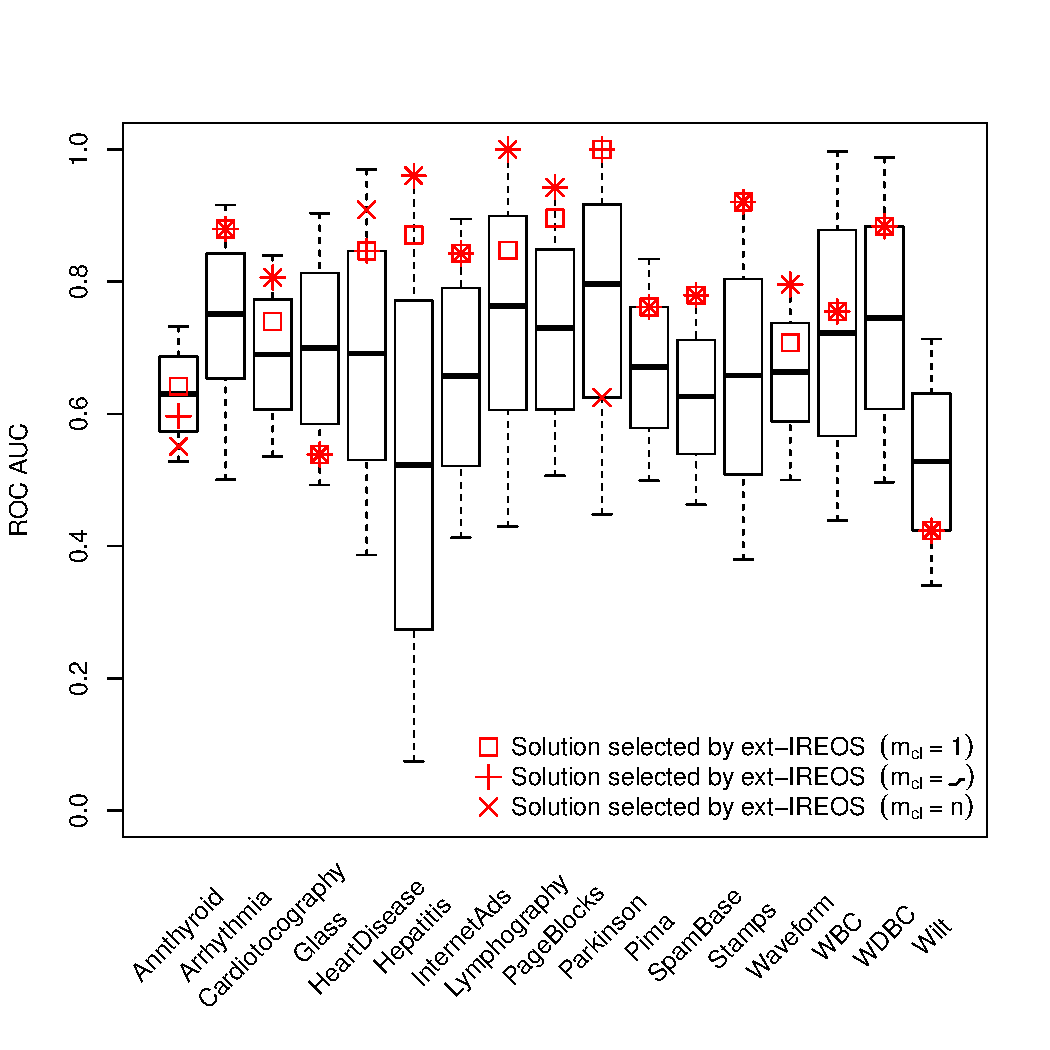
\includegraphics[width=\textwidth]{figs/boxplot.pdf}
\captionsetup{justification=centering}
\caption{Distribution of the ROC AUC values for all candidate solutions used in the experiments.}
\label{fig:boxplot}
\end{figure}

\newpage

\subsection{Computational experiments}

\subsubsection{Minimum number of $\gamma$}

%\begin{table}[h!]
%\centering
%\footnotesize
%\caption{Adaptive}
%\label{tab:adaptive}
%\begin{tabular}{|l|ll|lll|lll|lll|}
%\hline
%\multirow{2}{*}{Dataset} & \multicolumn{2}{c|}{Original} & \multicolumn{3}{c|}{0.1} & \multicolumn{3}{c|}{0.01} & \multicolumn{3}{c|}{0.001} \\ \cline{2-12} 
%                                   & Total        & Runtime     & Total  & Runtime  & Diff & Total  & Runtime  & Diff  & Total   & Runtime  & Diff  \\ \hline
%    Arrhythmia                     & 25600        & 0:13:45     &  4098 (16\%)  & 0:2:4 (15.11\%)   & 0.009805&        &          &       &         &          &       \\
%    Cardiotocography               & 173400       & 18:26:45    &  12468 & 1:16:54  & 0.00413 &        &          &       &         &          &       \\
%    Glass                          & 21400        & 0:2:1       &        &          &         &        &          &       &         &          &       \\
%    HeartDisease                   & 15700        & 0:0:55      &        &          &         &        &          &       &         &          &       \\
%    Hepatitis                      & 7000         & 0:0:7       &        &          &         &        &          &       &         &          &       \\
%    Lymphography                   & 14800        & 0:0:51      &        &          &         &        &          &       &         &          &       \\
%    PageBlocks                     & 513900       & 11:47:43    &        &          &         &        &          &       &         &          &       \\
%    Parkinson                      & 5000         & 0:0:3       &        &          &         &        &          &       &         &          &       \\
%    Pima                           & 52600        & 0:28:57     &        &          &         &        &          &       &         &          &       \\
%    SpamBase                       & 266100       & 4:9:0       &        &          &         &        &          &       &         &          &       \\
%    Stamps                         & 32500        & 0:7:3       &        &          &         &        &          &       &         &          &       \\
%    Waveform                       & 344300       & 13:37:13    &        &          &         &        &          &       &         &          &       \\
%    WBC                            & 22300        & 0:2:24      &        &          &         &        &          &       &         &          &       \\
%    WDBC                           & 367000       & 0:13:4      &        &          &         &        &          &       &         &          &       \\
%    Wilt                           & 481900       & 23:23:27    &        &          &         &        &          &       &         &          &       \\ \hline
%\end{tabular}
%\end{table}

\begin{table}[h!]
\centering
\footnotesize
\caption{Adaptive}
\label{tab:adaptive}
\begin{tabular}{|l|ll|lll|}
\hline
\multirow{2}{*}{Dataset} & \multicolumn{2}{c|}{Original} & \multicolumn{3}{c|}{0.01} \\ \cline{2-6} 
                                   & Total        & Runtime     & Total  & Runtime  & Diff   \\ \hline
Arrhythmia & 25600 & 0:13:56 & 4555.6 (17.8\%) & 0:2:43 (19.56\%)  &  0.00790  \\ 
Cardiotocography & 173400 & 18:26:45 & 13881.8 (8.01\%) & 1:34:39 (8.55\%)  &  0.01950  \\ 
Glass & 21400 & 0:2:9 & 2978.4 (13.92\%) & 0:0:34 (26.39\%)  &  0.00320  \\ 
HeartDisease & 15700 & 0:1:0 & 1796.2 (11.44\%) & 0:0:19 (32.41\%)  &  0.00813  \\ 
Hepatitis & 7000 & 0:0:7 & 1130.2 (16.15\%) & 0:0:2 (31.81\%)  &  0.00517  \\ 
Lymphography & 14800 & 0:0:55 & 1727.4 (11.67\%) & 0:0:16 (30.11\%)  &  0.00683  \\ 
PageBlocks & 513900 & 491:47:43 & 36811.8 (7.16\%) & 35:9:6 (7.15\%)  &  0.00361  \\ 
Parkinson & 5000 & 0:0:3 & 740.4 (14.81\%) & 0:0:1 (28.92\%)  &  0.00341  \\ 
Pima & 52600 & 0:30:43 & 5770 (10.97\%) & 0:4:32 (14.76\%)  &  0.01036  \\ 
SpamBase & 266100 & 124:9:0 & 35113 (13.2\%) & 17:59:15 (14.49\%)  &  0.00938  \\ 
Stamps & 32500 & 0:7:3 & 3228.4 (9.93\%) & 0:0:54 (12.77\%)  &  0.01213  \\ 
Waveform & 344300 & 157:37:13 & 39899 (11.59\%) & 21:34:18 (13.69\%)  &  0.01692  \\ 
WBC & 22300 & 0:2:32 & 3362.2 (15.08\%) & 0:0:34 (22.29\%)  &  0.00519  \\ 
WDBC & 36700 & 0:13:19 & 5017.4 (13.67\%) & 0:2:5 (15.68\%)  &  0.00887  \\ 
Wilt & 481900 & 359:23:27 & 34881.4 (7.24\%) & 26:58:52 (7.51\%)  &  0.01377  \\ 
 \hline
\end{tabular}
\end{table}

\begin{table}[h!]
\centering
\footnotesize
\caption{Adaptive}
\label{tab:adaptive}
\begin{tabular}{|l|lll|lll|}
\hline
\multirow{2}{*}{Dataset} & \multicolumn{3}{c|}{0.005} & \multicolumn{3}{c|}{0.001} \\ \cline{2-7} 
                                   & Total           & Runtime            & Diff     & Total           & Runtime            & Diff        \\ \hline
    Arrhythmia                     & 6104.8 (23.85\%) & 0:3:32 (25.38\%)  &  0.00266 & 8452.6 (33.02\%) & 0:4:44 (34.04\%)  &  0.00069          \\
    Cardiotocography               & 18755.6 (10.82\%) & 2:8:27 (11.61\%)  &  0.01734 & 29482 (17\%) & 3:22:27 (18.29\%)  &  0.01609           \\
    Glass                          & 3765 (17.59\%) & 0:0:38 (29.95\%)  &  0.00152 & 5239.8 (24.49\%) & 0:0:47 (36.65\%)  &  0.00028           \\
    HeartDisease                   & 2396.2 (15.26\%) & 0:0:21 (36.52\%)  &  0.00352 & 3536 (22.52\%) & 0:0:26 (44.32\%)  &  0.00072         \\
    Hepatitis                      & 1465.8 (20.94\%) & 0:0:2 (36.66\%)  &  0.00227 & 1987.2 (28.39\%) & 0:0:3 (43.19\%)  &  0.00041        \\
    Lymphography                   & 2330.8 (15.75\%) & 0:0:19 (34.55\%)  &  0.00358 & 3448 (23.3\%) & 0:0:23 (42.92\%)  &  0.00097         \\
    PageBlocks                     & 40901.8 (7.96\%) & 39:2:50 (7.94\%)  &  0.00199  & 50493.2 (9.83\%) & 48:9:0 (9.79\%)  &  5e-04          \\
    Parkinson                      & 957.6 (19.15\%) & 0:0:1 (32.74\%)  &  0.00165 & 1374 (27.48\%) & 0:0:1 (39.21\%)  &  0.00045        \\
    Pima                           & 8111.6 (15.42\%) & 0:5:55 (19.29\%)  &  0.00757 & 12057.4 (22.92\%) & 0:8:17 (26.99\%)  &  0.00635         \\
    SpamBase                       & 47637.8 (17.9\%) & 24:13:14 (19.51\%)  &  0.00363 & 65931 (24.78\%) & 33:14:10 (26.77\%)  &  0.00081       \\
    Stamps                         & 4312.4 (13.27\%) & 0:1:7 (15.86\%)  &  0.01015 & 6460.6 (19.88\%) & 0:1:33 (22.06\%)  &  0.00925       \\
    Waveform                       & 64058 (18.61\%) & 34:46:58 (22.07\%)  &  0.00512  & 90128.4 (26.18\%) & 49:3:33 (31.13\%)  &  0.00177       \\
    WBC                            & 4414.4 (19.8\%) & 0:0:41 (26.85\%)  &  0.00389 & 6051.2 (27.14\%) & 0:0:51 (33.86\%)  &  0.00344         \\
    WDBC                           & 7149 (19.48\%) & 0:2:49 (21.2\%)  &  0.00327 & 10172.2 (27.72\%) & 0:3:50 (28.84\%)  &  0.00207       \\
    Wilt                           & 39469 (8.19\%) & 30:35:16 (8.51\%)  &  0.01724 & 50346.2 (10.45\%) & 39:10:45 (10.9\%)  &  0.01141       \\ \hline
\end{tabular}
\end{table}

\subsubsection{Separability of the minimum number of observation}
\begin{table}[h!]
\footnotesize
\centering
\caption{Stopping}
\label{tab:stopping}
\begin{tabular}{|l|ll|ll|ll|}
\hline
\multirow{2}{*}{Dataset} & \multicolumn{2}{c|}{Original} &  \multicolumn{2}{c|}{Weights 0} & \multicolumn{2}{c|}{Stopping} \\ \cline{2-7} 
                                   & Total        & Runtime    & Total  & Runtime  & Total   & Runtime      \\ \hline
        Arrhythmia & 25600 & 0:13:56 & 11700 (45.7\%) & 0:6:11 (44.42\%) & 11233.33 (43.88\%) & 0:5:56 (42.64\%) \\
        Cardiotocography & 173400 & 18:26:45 & 86600 (49.94\%) & 9:14:12 (50.08\%) & 76576.67 (44.16\%) & 8:10:6 (44.28\%) \\
        Glass & 21400 & 0:2:9 & 9570 (44.72\%) & 0:0:55 (42.6\%) & 8943.333 (41.79\%) & 0:0:51 (39.85\%) \\
        HeartDisease & 15700 & 0:1:0 & 7800 (49.68\%) & 0:0:30 (51.12\%) & 7206.667 (45.9\%) & 0:0:28 (47.44\%) \\
        Hepatitis & 7000 & 0:0:7 & 3400 (48.57\%) & 0:0:3 (48.09\%) & 3163.333 (45.19\%) & 0:0:3 (44.65\%) \\
        InternetAds & 168200 & 1038:51:52 & 83970 (49.92\%) & 520:12:11 (50.07\%) & 80120 (47.63\%) & 496:25:4 (47.78\%) \\
        Lymphography & 14800 & 0:0:55 & 6490 (43.85\%) & 0:0:24 (44.1\%) & 6066.667 (40.99\%) & 0:0:22 (41.41\%) \\
        PageBlocks & 513900 & 491:47:43 & 234440 (45.62\%) & 224:9:21 (45.58\%) & 189413.3 (36.86\%) & 181:18:38 (36.87\%) \\
        Parkinson & 5000 & 0:0:3 & 2180 (43.6\%) & 0:0:1 (41.67\%) & 2033.333 (40.67\%) & 0:0:1 (38.98\%) \\
        Pima & 52600 & 0:30:43 & 23330 (44.35\%) & 0:13:37 (44.37\%) & 21966.67 (41.76\%) & 0:12:49 (41.78\%) \\
        SpamBase & 266100 & 124:9:0 & 132400 (49.76\%) & 61:47:29 (49.77\%) & 123600 (46.45\%) & 57:45:50 (46.53\%) \\
        Stamps & 32500 & 0:7:3 & 15900 (48.92\%) & 0:3:28 (49.1\%) & 14353.33 (44.16\%) & 0:3:7 (44.33\%) \\
        Waveform & 344300 & 157:37:13 & 154410 (44.85\%) & 70:57:10 (45.01\%) & 149543.3 (43.43\%) & 68:46:1 (43.63\%) \\
        WBC & 22300 & 0:2:32 & 9990 (44.8\%) & 0:1:5 (43.03\%) & 9610 (43.09\%) & 0:1:3 (41.47\%) \\
        WDBC & 36700 & 0:13:19 & 16390 (44.66\%) & 0:5:54 (44.35\%) & 15413.33 (42\%) & 0:5:33 (41.72\%) \\
        Wilt & 481900 & 359:23:27 & 240430 (49.89\%) & 179:14:18 (49.87\%) & 208526.7 (43.27\%) & 155:36:28 (43.3\%) \\ \hline
\end{tabular}
\end{table}

\subsubsection{Speed classifier up}
%\begin{table}[h!]
%%\begin{sidewaystable}
%\footnotesize
%\centering
%\caption{Nearest neighbor}
%\label{tab:nn}
%\begin{tabular}{|l|l|ll|ll|ll|ll|}
%\hline
%\multirow{2}{*}{Dataset} & \multicolumn{1}{c|}{Original} & \multicolumn{2}{c|}{100} & \multicolumn{2}{c|}{250} & \multicolumn{2}{c|}{500} & \multicolumn{2}{c|}{1000}  \\ \cline{2-10} 
%                         & Runtime  & Diff                    & Runtime       & Diff                         & Runtime       & Diff     & Runtime       & Diff      & Runtime            \\ \hline
    %Cardiotocography     & 178.76       & 0.0038 $\pm$ 0.0026     & 0.76          & 0.00094 $\pm$ 0.00065        & 4.05              & 0.00109 $\pm$ 0.00036    &  15.09        & 0.00048 $\pm$ 0.00011          &  58.97              \\
%    InternetAds          & 9509.71      & 0.0072 $\pm$ 0.0043     & 11.57         & 0.00473 $\pm$ 0.00267        & 210.68            & 0.00243 $\pm$ 0.00135        &  820.25   \\
    %PageBlocks           & 4694.77      & 0.0021 $\pm$ 0.0022     & 1.69          & 0.00343 $\pm$ 0.00104        & 9.36              & 0.00308 $\pm$ 0.00072         &  36.74        &   0.00245 $\pm$  0.00052       & 146.42                 \\
    %SpamBase             & 943.71       & 0.0198 $\pm$ 0.0055     & 2.11          & 0.01030 $\pm$ 0.00226        & 7.94              & 0.00553 $\pm$ 0.00118         &  31.55        & 0.00276 $\pm$ 0.00082       & 160.75              \\
    %Waveform             & 1459.54      & 0.0094 $\pm$ 0.0035     & 1.49          & 0.00344 $\pm$ 0.00127        & 8.09              & 0.00096 $\pm$ 0.00042        &  30.59        & 0.00013 $\pm$ 0.00013         & 119.46               \\
    %Wilt                 & 3500.33      & 0.0043 $\pm$ 0.0011     & 1.45          & 0.00441 $\pm$ 0.00039        & 8.07              & 0.00334 $\pm$ 0.00035         &  31.47        & 0.00248 $\pm$ 0.00031          & 124.74              \\ \hline
%\end{tabular}
%%\end{sidewaystable}
%\end{table}

\begin{table}[h!]
%\begin{sidewaystable}
\footnotesize
\centering
\caption{Nearest neighbor}
\label{tab:nn}
\begin{tabular}{|l|l|ll|ll|ll|}
\hline
\multirow{2}{*}{Dataset} & \multicolumn{1}{c|}{Original} & \multicolumn{2}{c|}{10} & \multicolumn{2}{c|}{50} & \multicolumn{2}{c|}{100}   \\ \cline{2-8} 
                         & Runtime  & Diff                    & Runtime       & Diff                         & Runtime       & Diff      & Runtime          \\ \hline
Cardiotocography  & 18:26:45 & 0.05651 $\pm$ 0.07093 & 0:0:11 & 0.01953 $\pm$ 0.02443 & 0:1:40 & 0.01725 $\pm$ 0.02395 & 0:4:54 \\ 
InternetAds  & 1038:51:52 & 0.03822 $\pm$ 0.07256 & 0:1:16 & 0.01213 $\pm$ 0.0165 & 0:19:40 & 0.01028 $\pm$ 0.00964 & 1:24:37 \\ 
PageBlocks  & 491:47:43 & 0.09086 $\pm$ 0.10938 & 0:0:20 & 0.04187 $\pm$ 0.06783 & 0:3:18 & 0.03835 $\pm$ 0.05949 & 0:10:51 \\ 
SpamBase  & 124:9:0 & 0.03691 $\pm$ 0.03992 & 0:0:15 & 0.02928 $\pm$ 0.02126 & 0:3:5 & 0.03367 $\pm$ 0.03464 & 0:11:16 \\ 
Waveform  & 157:37:13 & 0.03083 $\pm$ 0.01315 & 0:0:11 & 0.01309 $\pm$ 0.00637 & 0:2:44 & 0.00786 $\pm$ 0.00465 & 0:9:7 \\ 
Wilt  & 359:23:27 & 0.11055 $\pm$ 0.13974 & 0:0:17 & 0.05106 $\pm$ 0.05342 & 0:2:47 & 0.04109 $\pm$ 0.03445 & 0:9:4 \\  \hline
\end{tabular}
%\end{sidewaystable}
\end{table}

%\begin{table}[h!]
%%\begin{sidewaystable}
%\footnotesize
%\centering
%\caption{Nearest neighbor}
%\label{tab:nn}
%\begin{tabular}{|l|l|ll|ll|}
%\hline
%\multirow{2}{*}{Dataset} & \multicolumn{1}{c|}{Original} & \multicolumn{2}{c|}{250} & \multicolumn{2}{c|}{500}    \\ \cline{2-6} 
                         %& Runtime  & Diff                    & Runtime       & Diff                         & Runtime              \\ \hline
    %Cardiotocography     & 178.76       & 0.0038 $\pm$ 0.0026     & 0.76          & 0.00094 $\pm$ 0.00065        & 4.05                   \\
    %InternetAds          & 9509.71      & 0.0072 $\pm$ 0.0043     & 11.57         & 0.00473 $\pm$ 0.00267        & 210.68            \\
    %PageBlocks           & 4694.77      & 0.0021 $\pm$ 0.0022     & 1.69          & 0.00343 $\pm$ 0.00104        & 9.36                   \\
    %SpamBase             & 943.71       & 0.0198 $\pm$ 0.0055     & 2.11          & 0.01030 $\pm$ 0.00226        & 7.94                       \\
    %Waveform             & 1459.54      & 0.0094 $\pm$ 0.0035     & 1.49          & 0.00344 $\pm$ 0.00127        & 8.09                     \\
    %Wilt                 & 3500.33      & 0.0043 $\pm$ 0.0011     & 1.45          & 0.00441 $\pm$ 0.00039        & 8.07              \\ \hline
%\end{tabular}
%%\end{sidewaystable}
%\end{table}


\begin{table}[h!]
%\begin{sidewaystable}
\footnotesize
\centering
\caption{Nearest neighbor}
\label{tab:nn}
\begin{tabular}{|l|l|ll|}
\hline
\multirow{2}{*}{Dataset} & \multicolumn{1}{c|}{Original} & \multicolumn{2}{c|}{Combined approaches}    \\ \cline{2-4} 
                         & Runtime  & Runtime                    &    Diff               \\ \hline
Arrhythmia  & 0:13:56 & 0:0:14 (1.79\%)  &  0.00459  \\ 
Cardiotocography  & 18:26:45 & 0:0:17 (0.03\%)  &  0.00869  \\ 
Glass  & 0:2:9 & 0:0:3 (2.96\%)  &  0.00156  \\ 
HeartDisease  & 0:1:0 & 0:0:3 (5.55\%)  &  0.00282  \\ 
Hepatitis  & 0:0:7 & 0:0:1 (17.34\%)  &  0.00222  \\ 
InternetAds  & 1038:51:52 & 0:13:19 (0.02\%)  &  0.01042  \\ 
Lymphography  & 0:0:55 & 0:0:2 (4.78\%)  &  0.00337  \\ 
PageBlocks  & 491:47:43 & 0:0:24 (0\%)  &  0.0018  \\ 
Parkinson  & 0:0:3 & 0:0:0 (16.96\%)  &  0.00187  \\ 
Pima  & 0:30:43 & 0:0:7 (0.42\%)  &  0.00705  \\ 
Stamps  & 0:7:3 & 0:0:4 (1.07\%)  &  0.0035  \\ 
SpamBase  & 124:9:0 & 0:1:34 (0.02\%) & 0.02389 \\  
WBC  & 0:2:32 & 0:0:4 (2.92\%)  &  0.00464  \\ 
WDBC  & 0:13:19 & 0:0:7 (0.88\%)  &  0.00658  \\ 
Wilt  & 359:23:27 & 0:0:25 (0\%)  &  0.00316  \\  \hline
\end{tabular}
%\end{sidewaystable}
\end{table}
%\subsubsection{Model selection \& correlation}


\end{document} 
